\documentclass[10pt]{article}
\usepackage[a4paper,margin=18mm]{geometry}
\usepackage{amsmath,amssymb,graphicx,hyperref}
\hypersetup{colorlinks=true,urlcolor=blue}
\setlength{\parindent}{0pt}\setlength{\parskip}{6pt}
\begin{document}
\begin{center}\Large One retained row per independent query\\[3pt]
\normalsize Contract addendum, 16 November 2026 --- PCC unverified\end{center}
The frozen private-coefficient draft did not explicitly cap retained rows
per query. Its independent-tag argument requires \textbf{at most one retained
checked relation per query with fresh private coefficients}. Choose that row
without using its tags or their seed. Identical targets or rows from different
queries remain allowed. The actual point/selection bridge is still open.
[pcc:unverified]

\begin{center}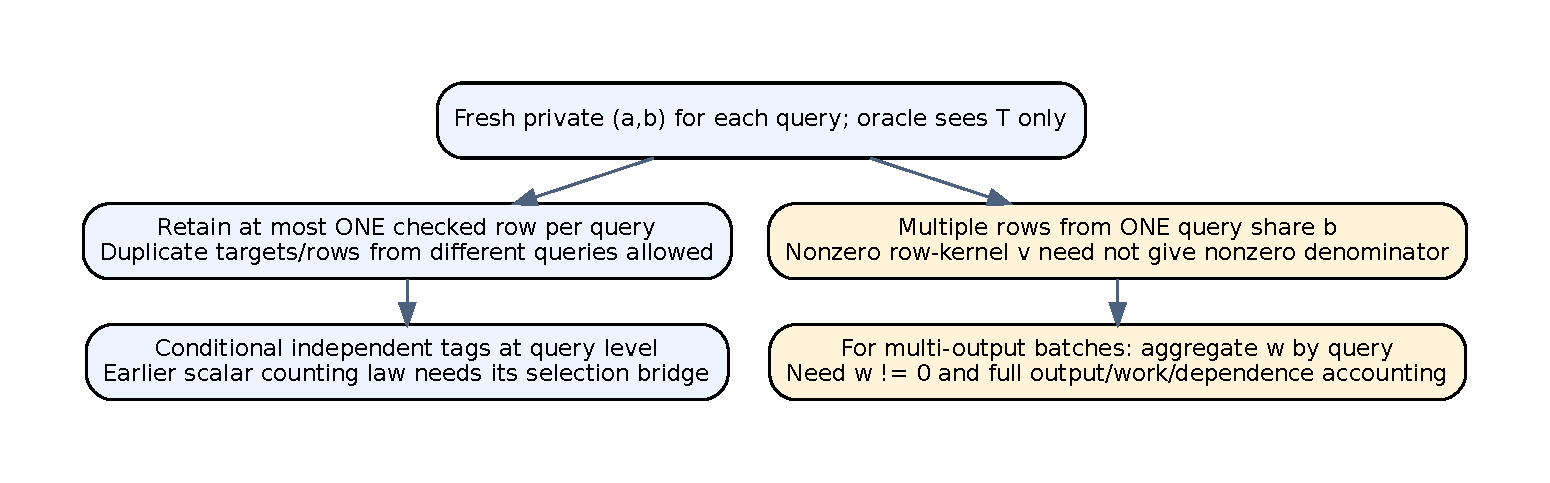
\includegraphics[width=0.98\linewidth,height=75mm,keepaspectratio]{pipeline.pdf}\end{center}

\textbf{Concrete witness.} Over $\mathbb F_5$, put
\[
C=\begin{pmatrix}1\\1\end{pmatrix},\qquad v=(1,-1),\qquad t=(b,b).
\]
For every $b$, $v\ne0$, $v^TC=0$ and $v\cdot t=b-b=0$.
The new SharedQueryCounterexample Lean module checks this concrete instance
using existing Mathlib laws. The vector is tag-blind; shared query tags alone
cause cancellation. This refutes the extension that silently treats
same-query rows as independent. It is not an exclusion of multi-output
algorithms or a new curve-decomposition result. [pcc:unverified]

\textbf{Query aggregation.} If row $i$ belongs to query $\pi(i)$, then
\[
\beta=\sum_i v_i b_{\pi(i)}=\sum_j w_j b_j,
\qquad w_j=\sum_{i:\pi(i)=j}v_i.
\]
The earlier annihilator-count law needs nonzero, tag-independent $w$ at the
query level. Nonzero $v$ is insufficient. Arbitrary grouping, selection and
probability bridges are outside the concrete F5 certificate. [pcc:unverified]

\textbf{Cost scope.} Success probability is capped at one; returned-row
counts may exceed one. The earlier $P+BD/y+L$ and numeric rational-envelope
examples are the at-most-one-retained-row model. Multi-output batching must
charge total computation, all output/checking work and query dependencies,
and establish its aggregate-kernel condition. It remains a research option.
[pcc:unverified]

Original reports, source/manifest contexts and theorem statements retain
their exact bytes. This addendum clarifies their open application contracts;
it does not establish a decomposition-cost bound or changed attack exponent.
[pcc:unverified]

\textbf{Sources.} Source-linked REPORT.md; the frozen private-coefficient
proposal; existing CryptoLean.SingleRelation label/recovery laws;
\href{https://people.maths.ox.ac.uk/petit/files/16PKC_primeECDLP.pdf}{PKM2016,
section2.1 and Algorithm1}. No novelty is asserted.
\end{document}
